\apendice{Plan de Proyecto Software}

\section{Introducción}

Cuando queremos hablar de la realización de proyecto, nos encontramos con una fase primordial, que es es la planificación. En esta etapa se estiman los tiempos y el presupuesto del proyecto. 

Para hablar de estas estimaciones, se debe tener en cuenta las partes que realizan el proyecto estén de acuerdo con todas las ideas planteadas. Se dividirán en dos partes: 

\begin{itemize}
	\item \textit{Planificación temporal}: hablaremos de todas las reuniones realizadas y además comprobaremos si los tiempos de la realización del proyecto son óptimos.
	\item \textit{Estudio de viabilidad}: intentaremos decidir si el proyecto fue bien planteado o falló algo en la ejecución, dentro de este estudio, tendremos dos tipos de viabilidad:
	\begin{enumerate}[a]
		\item \textit{Económica}: explicaremos los costes y posibles beneficios del proyecto.
		\item \textit{Legal}: estudiaremos las leyes que tuvieran que ver con nuestro proyecto.
	\end{enumerate}
\end{itemize}

\section{Planificación temporal}

Como hablamos en la memoria, utilizaremos una metodología Scrum. Las características de este método son:

\begin{itemize}
	\item Utilizaremos una estrategia de sprint para esta metodología, dividiremos el trabajo en intervalos de un tiempo y así observaremos su desarrollo.
	\item Con cada sprint se planifican las tareas a realizar y el tiempo en el que desarrollaremos el trabajo. En general las reuniones fueron cada dos semanas.
	\item Al finalizar el sprint, realizaremos una reunión mediante videollamada o asistiendo personalmente a León.
\end{itemize}

El inicio del proyecto comienza con una reunión con el tutor Pablo Tejedor García mediante una llamada telefónica, en ella hablamos un poco acerca del porqué de la elección de este trabajo y cuales serán los objetivos del proyecto y las opciones que tendremos para realizarlas. 

El tutor de HP, me comentó que es un proyecto de investigación,  con una tecnológica nunca utilizada anteriormente en dicha empresa, el mundo Blockchain.


\subsection{Sprint 1 (24/10/18 - 16/11/18)}

En la primera reunión realizada hablamos de los objetivos y la realización de la siguiente tarea:

\begin{itemize}
	\item Lectura del libro \textit{``Scrum desde las trincheras''} \cite{libro}.
	\item Realización del curso ``CrytoZombies''.
\end{itemize}

Se calculan 30 horas de trabajo.

\subsection{Sprint 2 (16/11/18 - 15/01/19)}

Primeramente hablamos de la conclusión del sprint anterior y cómo fue la primera toma de contacto con un lenguaje nunca usado anteriormente.

Para esta segunda reunión se propusieron las siguientes tareas:
\begin{itemize}
	\item Resumen del libro leído en el sprint anterior.
	\item Creación de un \textit{smart contract}, con cierta funcionalidad en modo local.
	\item Realización de programas en Visual Studio, para la realización de pequeños archivos.
	\item Investigación de Truffle como entorno, ya que es una plataforma que nos permitirá desarrollar \textit{smart contracts} y desplegarlos para poder consumirlos desde un frontEnd.
\end{itemize}

Se calculan 45 horas de trabajo.

\subsection{Sprint 3 (15/01/19 - 12/02/19)}

Para esta nueva tarea se proponen las siguientes tareas:

\begin{itemize}
	\item Documentación somera de Truffle. Necesitamos una pequeña guía de que es, cómo instalarlo y qué funcionalidades proporciona Truffle para la memoria del Proyecto.
	\item Desarrollo de un \textit{smart contract} sencillo con la plataforma Truffle. Un pequeño \textit{smart contract} funcional con el que podamos empezar a trabajar.
	\item Desarrollo de una pequeña aplicación de escritorio o web (a decisión del alumno) en Visual Studio 2017 que disponga de una sola pantalla y elementos para interactuar con la capa de abajo donde se situará el \textit{smart contract} desplegado.
\end{itemize}

Se calculan 40 horas de trabajo.

\subsection{Sprint 4 (12/02/19 - 28/02/19)}

Para la cuarta reunión en el proyecto se habló de la sesión anterior, en la cual comprobamos el guión de Truffle. Realizamos la ejecución de los \textit{smart contract} realizados en el lenguaje Solidity y visualización de los proyectos creados en la aplicación Visual Studio 2017.

Las tareas a realizar para la siguiente sesión serán: 

\begin{itemize}
	\item Realización de un guión con la información a poner en la memoria.
	\item Investigación sobre web3.js (conexión entre Visual Studio y Ethereum).
	\item Creación de página de autobuses para realizar un simulacro de la página final, pero con modo local (Ganache).
\end{itemize}

Se calculan 52 horas de trabajo.

\subsection{Sprint 5 (28/02/19 - 29/03/19)}

Comentamos los problemas que surgieron en la sprint 4.

El principal quebradero de cabeza del sprint anterior fue la conexión entre web3.js, no sabíamos dar con el error ya que cuando probamos la aplicación nueva de autobuses con Ganache (modo Local) la conexión era perfecta y realizaba el cambio de divisa sin ningún problema.

Intentamos buscar alternativas cuando teníamos el error con web3.js (en modo red privada global o red principal Ethereum). Me propuso realizar la aplicación olvidándonos de la conexión con Ethereum y realizar una base de datos para poder mostrar todo desde ahí.

Pero seguimos indagando e intentamos realizarlo, pero con otras propuestas de editores de código.

\begin{itemize}
	\item Realizar conexión entre metamask y un editor de código, con web3.
	\item Desarrollar el guión creado del sprint anterior.
\end{itemize}

Se calculan 25 horas de trabajo.

\subsection{Sprint 6 (29/03/19 - 08/04/19)}

Esta reunión se realizo en León de forma presencial y en ella comentamos el guion y la posibilidad de modificar algún punto para la mayor compresión de esta nueva tecnología.

Expliqué a Pablo el editor nuevo usado para la conexión de Ethereum y nuestro editor, y conseguimos la conexión entre ambos medios; pudiendo así realizar los \textit{smart contract}, tanto en red local, privada y global (esto lo conseguimos en Visual Stuido Code).

Una vez teníamos la conexión realizada ya teníamos una gran parte del objetivo del proyecto realizado.

Los siguientes objetivos a tratar para hablar de ellos en el siguiente sprint fueron:

\begin{itemize}
	\item Creación de la pagina web, con las diferentes pantallas y la conexión entre ellas que fuera correctas.
	\item Buscar una base de datos para nuestro proyecto. 
	\item Documentar la memoria.
\end{itemize}

Se calculan 60 horas de trabajo.
	
\subsection{Sprint 7 (08/04/19 - 02/05/19)}

Comentamos las páginas creadas de nuestra web, comprobamos la funcionalidad con metamask y este con Ethereum. La conexión era buena, ahora queda realizar los css y dejar la página armonizar todas las páginas. 

La base de datos que realizamos es la de MySql, se encarga de almacenar a los usuarios y los datos enviados a la red Ethereum.

Para el siguiente sprint los objetivos serían:

\begin{itemize}
	\item Armonización de la página web en todas sus páginas.
	\item Creación de página de Administrador que pueda manejar a todos los usuarios que tenemos registrados.
	\item Poder seleccionar un avatar cuando creamos usuario.
\end{itemize}

Se calculan 27 horas de trabajo.


\subsection{Parón de los Sprint (02/05/19 - 23/10/19)}

En esta reunión comente la idea de que me iba de viaje a Estados Unidos y la fecha de ir no sería posible la entrega del Tfg de modo presencia, y que era demasiado tarde para poder cambiarlo a modo on-line, les hable de mi idea de continuar con el mismo Tfg para entregar en la primera convocatoria del curso 2019/2020.

Lo que supuso que en este parón hasta volver de Estados Unidos no realizaramos ningún Sprint ni hubiera avances en el desarrollo del proyecto.


\subsection{Sprint 8 (23/10/19 - 18/11/19)}

En esta reunión hablamos sobre pequeñas funcionalidades de nuestra página que se podrían añadir:

\begin{itemize}
	\item Introducción de un código \textit{captha} cuando se registra el usuario.
	\item Creación de una nueva página: ¿Has olvidado la contraseña?
	\item Modificación de la visualización de todos los productos pedidos.
	\item Comenzar con el apartado de los anexos, explicación de cada sprint.
\end{itemize}

También nos dimos cuenta de que la red Ropsten se nos estaba quedando sin Ether y pensamos en suprimir el dinero cada vez que se realiza el \textit{smart contract} y dejar solamente el gas de cada transacción.

Se calculan 45 horas de trabajo.

\subsection{Sprint 9 (18/11/19 - 12/12/19)}

Primeramente hablamos de la reunión anterior y comentamos la dificultad encontrada en realizar la función del \textit{captha} y ¿Has olvidado la contraseña?, ya que al ser en modo local y no tener un dominio, tendríamos que realizarlo de otras maneras.

El objetivo para la décima reunión es:

\begin{itemize}
	\item Mejorar los apartados resumen, introducción y concretos teóricos de la memoria.
	\item Investigar la opción de realizar el captha y ¿has olvidado la contraseña? mediante otro método.
	\item Continuar con los anexos.
\end{itemize}

Se calculan 37 horas de trabajo.


\subsection{Sprint 10 (12/12/19 - 20/12/2019)}

En la décima reunión hablamos de lo siguiente:

\begin{itemize}
	\item Finalizar de la página Web.
	\item Intentar crear un ejecutable para nuestra aplicación.
	\item Finalizar la memoria y anexos.
\end{itemize}

Se calculan 55 horas de trabajo.

\subsection{Sprint 11 (20/12/2019 - entrega proyecto)}

En la última reunión hablamos de lo siguiente:

\begin{itemize}
	\item Comprobar todas la funcionalidad de la web y la conexión con la red Ethereum.
	\item Decisión de realizar la entrega desde la cuenta Localhost.
	\item Revisar la memoria y anexos.
	\item Descargar todos los documentos para visualizar la información y ver que es correcta. Así evitaremos que se pueda encontrar imágenes cortadas o textos mal indexados.
\end{itemize}


\subsection{Resumen}

En la siguiente tabla \ref{tabla:tabla1}, veremos la distribución del tiempo en las diferentes tareas que se realizarón  para la elaboración de este proyecto, cada tarea se expresa en horas:

\begin{table}[H]
	\begin{center}
		\begin{tabular}{|l|l|}
		\hline
			Tarea a realizar & Tiempo(horas)\\ 
			\hline \hline
			Programación & 150 \\ \hline
			Investigación & 105 \\ \hline
			Documentación & 90 \\ \hline
			Revisión y corrección de errores & 54\\ \hline
			Reuniones & 17 \\ \hline
			Total & 416 \\ \hline
		\end{tabular}
	\caption{Tiempo empleado en el proyecto.}
	\label{tabla:tabla1}
	\end{center}
\end{table}

En el siguiente gráfico \ref{ref:horas}, observaremos el tiempo empleado estructurado en el desarrollo del proyecto.

\begin{figure}
    \centering
    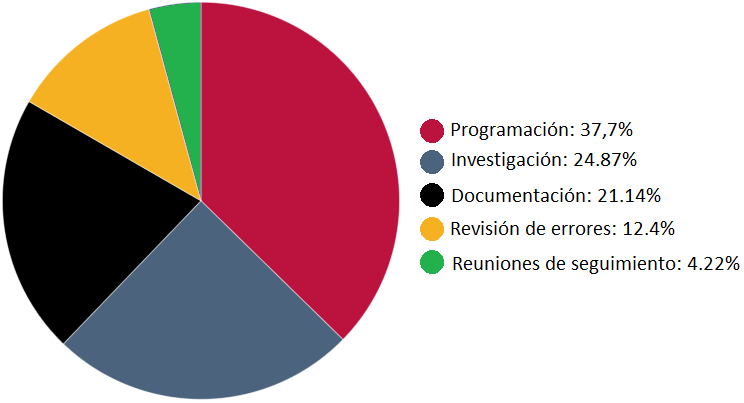
\includegraphics[width=0.80\textwidth]{quesitoTiempo}
    \caption{Gráfico de las horas empleadas en el proyecto}
    \label{ref:horas}
\end{figure}
 
A continuación explicaremos, el proceso de los sprint con una breve explicación de las tareas que se realizan en cada una de ellas \ref{tabla:sprint0} \ref{tabla:sprint2} 

\begin{table}[H]
\begin{tabular}{|p{1.5cm}|p{1.5cm}|p{5cm}}
\hline
\textbf{Sprint- horas} &  \textbf{Fechas de las tareas} & \multicolumn{1}{l|}{\textbf{Concepto}}                                                                                    \\ \hline
Sprint 1: 30 horas       & 24/10/18 24/10/18           &                                                                                                                   \\ \hline
               & Tarea 1             & \multicolumn{1}{p{9.2cm}|}{Conocer al tutor empresarial y comentar los objetivos y decisión de la elección de este TFG.} \\ \hline
                         & Tarea 2                       & \multicolumn{1}{p{9.2cm}|}{Lectura del libro “Scrum desde las trincheras".}                                              \\ \hline
                         & Tarea 3                       & \multicolumn{1}{p{9.2cm}|}{Realización del curso “CrytoZombies”.}                                                        \\ \hline
Sprint 2: 45 horas       & 16/11/18 15/01/19           & \multicolumn{1}{p{9.2cm}|}{}                                                                                             \\ \hline
                         & Tarea 1                       & \multicolumn{1}{p{9.2cm}|}{Puesta en común de las tareas del Sprint anterior.}                                  \\ \hline
                         & Tarea 2                       & \multicolumn{1}{p{9.2cm}|}{Creación de un smart contract, con cierta funcionalidad en modo local}               \\ \hline
                         & Tarea 3                       & \multicolumn{1}{p{9.2cm}|}{Comienzo con visual studio y con herramienta Truffle}                                \\ \hline 

Sprint 3: 40 horas       & 15/01/19 12/02/19           & \multicolumn{1}{p{9.2cm}|}{}                                                                                             \\ \hline
                         & Tarea 1                       & \multicolumn{1}{p{9.2cm}|}{Documentación de truffle para creacción de smart contract}                           \\ \hline
                         & Tarea 2                       & \multicolumn{1}{p{9.2cm}|}{Creacion de programas Visual Studio y comprobar su conexión con ethereum}            \\ \hline
Sprint 4: 52 horas       & 12/02/19 28/02/19           & \multicolumn{1}{l|}{}                                                                                             \\ \hline
                         & Tarea 1                       & \multicolumn{1}{p{9.2cm}|}{Creación de guión para la futura memoria.}                                                    \\ \hline
                         & Tarea 2                       & \multicolumn{1}{p{9.2cm}|}{Investigación de Web3.js, con creación de página para ver su funcionamiento.}                 \\ \hline
                         
              \end{tabular}
              \caption{realizadas en cada sprint}
\label{tabla:sprint0}
\end{table}       
         
\begin{table}[H]
\begin{tabular}{|p{1.5cm}|p{1.5cm}|p{5cm}}
\hline
\textbf{Sprint- horas} &  \textbf{Fechas de las tareas} & \multicolumn{1}{l|}{\textbf{Concepto}}                                                                                    \\ \hline
Sprint 5: 25 horas       & 28/02/19 29/03/19           & \multicolumn{1}{l|}{}                                                                                             \\ \hline
                         & Tarea 1                       & \multicolumn{1}{p{9.2cm}|}{Desarrollo del guión del Sprint 4.}                                                           \\ \hline
                         & Tarea 2                       & \multicolumn{1}{p{9.2cm}|}{Comprender y enlazar la herramienta Metamask con web3}                                        \\ \hline
Sprint 6: 60 horas       & 29/03/19 08/04/19           & \multicolumn{1}{l|}{}                                                                                             \\ \hline
                         & Tarea 1                       & \multicolumn{1}{p{9.2cm}|}{Comienzo de la página web final.}                                                             \\ \hline
                         & Tarea 2                       & \multicolumn{1}{p{9.2cm}|}{Buscar una base de datos para almacenar usuarios.}                                            \\ \hline
                         & Tarea 3                       & \multicolumn{1}{p{9.2cm}|}{Documentar la memoria}                                                                        \\ \hline
Sprint 7: 27 horas       & 08/04/19 02/05/19           & \multicolumn{1}{p{9.2cm}|}{}                                                                                             \\ \hline
                         & Tarea 1                       & \multicolumn{1}{p{9.2cm}|}{Creación de página de Administrador}                                                          \\ \hline
                         & Tarea 2                       & \multicolumn{1}{p{9.2cm}|}{Crear avatar para los usuarios.}                                                              \\ \hline
                         & Tarea 3                       & \multicolumn{1}{p{9.2cm}|}{Armonizar la página web}                                                                      \\ \hline
                       

Sprint pausa             & 02/05/19 23/10/19                               & \multicolumn{1}{p{9.2cm}|}{}                                                                                             \\ \hline
                         &                               & \multicolumn{1}{p{9.2cm}|}{Parón por motivo de trabajo en el extranjero}                                                                                             \\ \hline
                 
                         
Sprint 8: 45 horas       & 23/10/19 18/11/19           & \multicolumn{1}{l|}{}                                                                                             \\ \hline
                         & Tarea 1                       & \multicolumn{1}{p{9.2cm}|}{Introducción de un código captha y página ¿has olvidado contraseña?}                          \\ \hline
                         & Tarea 2                       & \multicolumn{1}{p{9.2cm}|}{Modificación de alguna página.}                                                               \\ \hline
Sprint 9: 37 horas       & 18/11/19 12/12/19           & \multicolumn{1}{l|}{}                                                                                             \\ \hline
                         & Tarea 1                       & \multicolumn{1}{p{9.2cm}|}{Mejorar memoria y continuar anexos.}                                                 \\ \hline
                         & Tarea 2                       & \multicolumn{1}{p{9.2cm}|}{Insertar captha mediante otro método.}                                               \\ \hline
%                         \end{tabular}
%\label{tabla:sprint1}
%\end{table}
%
%\begin{table}[H]
%\begin{tabular}{|p{1.5cm}|p{1.5cm}|p{5cm}}
%\hline
%\textbf{Sprint- horas} &  \textbf{Fechas de las tareas} & \multicolumn{1}{l|}{\textbf{Concepto}}                                                                                    \\ \hline  
Sprint 10: 55 horas      & 12/12/19 20/12/19         & \multicolumn{1}{l|}{}                                                                                             \\ \hline
                         & Tarea 1                       & \multicolumn{1}{p{9.2cm}|}{Finalizar de la página Web.}                                                                  \\ \hline
                         & Tarea 2                       & \multicolumn{1}{p{9.2cm}|}{Investigar como crear un ejecutable.}                                                         \\ \hline
Sprint 11:               & 20/12/19  entrega  & \multicolumn{1}{l|}{}                                                                                             \\ \hline
                         & Tarea 1                       & \multicolumn{1}{p{9.2cm}|}{Comprobar todas la funcionalidad de la web y la conexión con la red Ethereum.}                \\ \hline
                         & Tarea2                        & \multicolumn{1}{p{9.2cm}|}{Entrega del proyecto desde Localhost.}                                                        \\ \hline
\end{tabular}
\caption{Tareas realizadas en cada sprint}
\label{tabla:sprint1}
\end{table}

El el siguiente gráfico \ref{ref:gantt} se podrá observar, el Diagrama de Gantt \cite{gantt} es una herramienta gráfica cuyo objetivo es exponer el tiempo de dedicación previsto para diferentes tareas o actividades a lo largo de un tiempo total determinado. El diagrama se ha creado gracias a las herramientas que ofrece la siguiente pagina web \cite{ganttGrafico}

\begin{figure}[H]
    \centering
    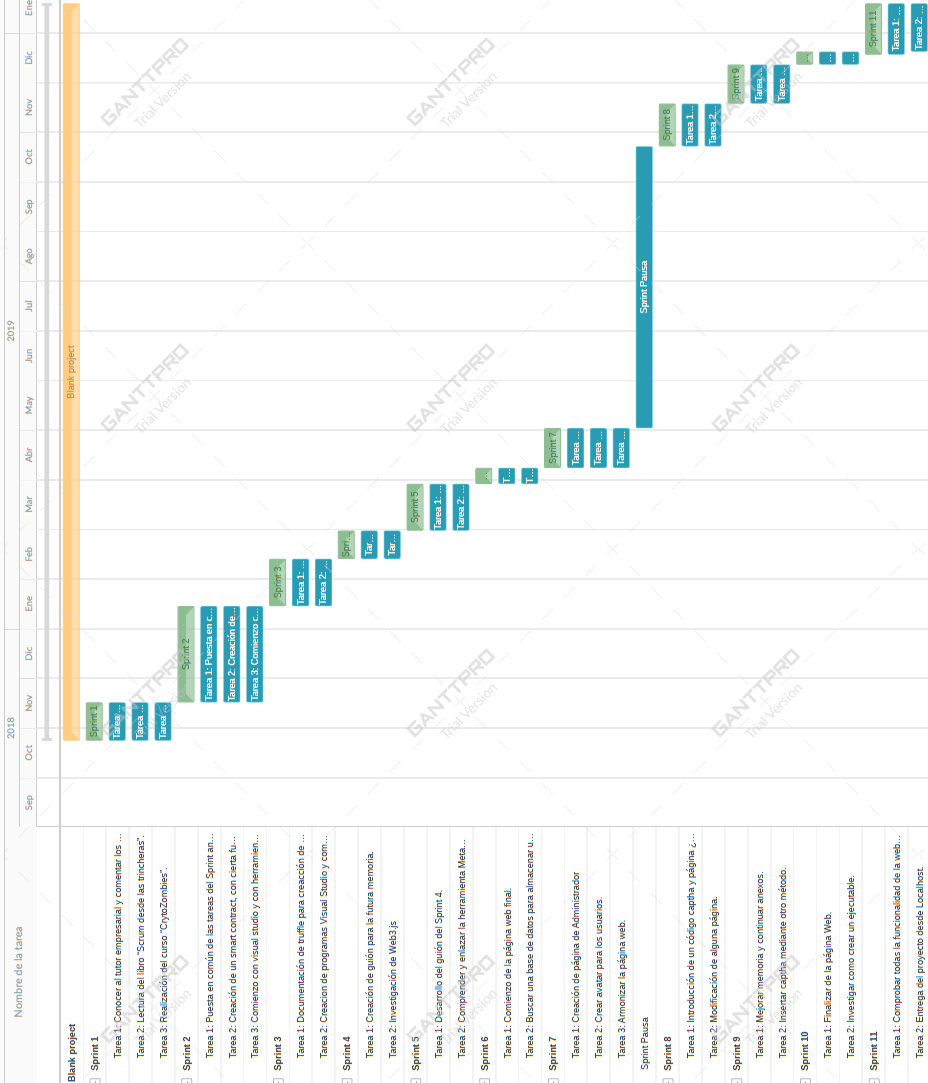
\includegraphics[width=1.00\textwidth]{dig-gantt2}
    \caption{Diagrama de Gantt}
    \label{ref:gantt}
\end{figure}

\section{Estudio de viabilidad}

En este apartado nos dispondremos a analizar los puntos de  viabilidad económica y legal, con esto podremos observar si es beneficioso o no realizar el proyecto.

\subsection{Viabilidad económica}

En el primer subapartado, expondremos costes y beneficios que tendría la realización de este proyecto en el entorno empresarial.

\subsubsection{Coste de personal}

La realización de este trabajo ha sido llevada acabo por un desarrollador junior durante 8 meses, con base en estos datos calcularemos los siguientes parámetros:

Se estima que el sueldo medio de un programador junior en España esta entre los 14.000 y los 16.000 euros brutos anuales. Para este calculo tomaremos la cifra de 14.000 euros , a este coste tendremos que añadir la parte proporcional a la seguridad social, la cual corre a cargo de la empresa, que es el 23.6\% del sueldo del empleado \cite{seguirdadSocial}. 

La estimación media para la realización del proyecto es de 13 horas semanales, compatibilizando el tiempo con la finalización del grado en ingeniería informática y realización de trabajo externo. Lo que hace un total de 416 horas empleadas en la elaboración del proyecto (8 meses * 4 semanas/mes * 13 horas/semana).


\begin{table}[h]
	\begin{center}
		\begin{tabular}{llll}
			Concepto              & Trabajador & Empresa &  \\ \hline
			Contingencias comunes & 4,7\%      & 23,6\%  &  \\ \hline
			Desempleo             & 1.55\%     & 5,5\%   &  \\ \hline
			Formación profesional & 0,1\%      & 0.6\%   &  \\ \hline 
			Garantía social       & 0          & 0.2\%   &  \\ \hline     
			TOTAL                 & 6.35\%     & 29.9\% &   \\
		\end{tabular}
	\caption{Gastos de la seguridad social}
	\label{tabla:tabla2}
	\end{center}
\end{table}

A continuación calculamos el precio hora que cobraremos, para luego calcular el salario con la seguridad social.

\begin{table}[htbp]
	\begin{center}
		\begin{tabular}{llll}
			Concepto                           & Coste (Euros)\\ \hline
			Salario anual              		   & 14.000 \\ 
			Salario mensual					   & 1166.66\\ 
			Salario a la hora                  & 7.29  \\ 
			Suelo sin seguridad social 		   & 3033.33 \\
			Sueldo con seguridad social (23.6\%)& \textbf{3749.19} \\\hline
		\end{tabular}
	\caption{Coste del empleado}
	\label{tabla:tabla3}
	\end{center}
\end{table}

Dentro de estos costes tendremos que añadir el coste del tutor.

\subsubsection{Coste informático}

Dentro de esta rama, los podremos dividir en dos clases que serán las siguientes:
 
\paragraph{Coste de hardware}

Para la realización de este proyecto, únicamente se tendrá en cuenta el coste del ordenador utilizado, el coste del ordenador ronda entre los 700 y los 900 euros.
El ordenador con el cual se ha realizado el proyecto tiene una antigüedad de 5 años y se estima un uso de vida total de 8 años y tiene un valor de 750 euros. El tiempo de empleo para este trabajo ha sido de 8 meses, por lo tanto el coste amortizado de estos meses será de 116.69 euros.

También se podrían sumar otros gastos como son luz, Internet, material de oficina pero son despreciables y por eso no se incluyen en esté calculo.

\paragraph{Coste de software}

Para la realización del proyecto, todos los programas, bibliotecas y herramientas empleadas son de software libre y gratuito. En caso de haber tenido alguna versión de pago, empleábamos la version anterior o su versión de prueba.

\subsubsection{Coste de total}

Para concluir, tendremos los siguientes costes, durante el tiempo dedicado a este proyecto, salario del empleado con la seguridad social incluida y costes informáticos.

\begin{table}[H]
	\begin{center}
		\begin{tabular}{llll}
			Concepto              & Coste (Euros)\\ \hline
			Salario total         & 3749.19  \\ \hline	
			Costes informáticos	  & 116.69    \\ \hline
			TOTAL                 & 3862.88     \\
		\end{tabular}
	\caption{Coste del empleado}
	\label{tabla:tabla4}
	\end{center}
\end{table}

El precio total del proyecto serían 3862.88 euros, esto teniendo en cuenta, que faltaría indicar de sumar el salario del tutor.

\subsubsection{Beneficio}

En cuanto a los beneficios serían inexistentes, ya que serían indirectos y se plantearía como una aplicación de uso propio para HP, con ello ayudaría en el desarrollo de la tecnología Blockchain, teniendo en cuenta en el auge de esta herramienta cada vez más usada en todos las industrias podrá ser adaptado para futuras operaciones con diferentes clientes. Asi los beneficios serían 100\% indirectos. 


\subsection{Viabilidad legal}

En este último apartado expondremos la viabilidad en el ámbito legal, hablaremos sobre las licencias software que empleamos en el desarrollo del mismo.

Se define una licencia software \cite{licencia} como un contrato mediante el cual una persona recibe de otra el derecho de uso, copia, distribución, estudio y modificación de varios de sus bienes, (normalmente de carácter intelectual), pudiéndose realizar un pago de una determinada cantidad por el uso de los mismos.

Los programas y herramientas utilizadas durante el desarrollo de este proyecto han sido de licencia abierta o de uso libre y gratuito (Solidity, HTML, PHP, Remix, Ganache \ldots). Esto es gracias a la licencia MIT ( \textit{Massachusetts Institute of Technology}) \cite{MIT}, la cual da libertad para poder usar el software libremente y con ello exime de responsabilidad a la parte creadora de las herramientas.
	
El proyecto se ha realizado en colaboración con HP SCDS, por esta razón el software resultante está bajo licencia copyright de la empresa. Asimismo, el código fuente será propiedad de HP SCDS y de la universidad de Burgos y podrá estar también bajo licencia copyright.
